\documentclass[]{elsarticle}

\usepackage{lineno,hyperref}
\modulolinenumbers[5]

%%%%%%%%%%%%%%%%%%%%%%%%%%%%%%%%%%%%%%%%%%%%%%%%%%%%%%%%%%
\usepackage{graphicx}
\graphicspath{{./}}
\usepackage{algorithm}
\usepackage{algorithmic}
\usepackage{textcomp}
%%%%%%%%%%%%%%%%%%%%%%%%%%%%%%%%%%%%%%%%%%%%%%%%%%%%%%%%%%
\usepackage{booktabs}
\usepackage{longtable}
\usepackage[smaller]{acronym}
\usepackage{amsmath}
\usepackage{nicefrac}
\usepackage{xspace}
\usepackage{rotating}
\usepackage{url}
%\usepackage{ulem}

\newcommand{\ver}[1]{\textcolor{orange}{#1}}


\newcommand*{\eg}{e.g.\@\xspace}
\newcommand*{\ie}{i.e.\@\xspace}
\newcommand{\FL}[1]{\textsc{fl#1}}
\newcommand{\PELT}{\textsc{pelt}}
\newcommand{\DBSCAN}{\textsc{dbscan}}
%%%%%%%%%%%%%%%%%%%%%%%%%%%%%%%%%%%%%%%%%%%%%%%%%%%%%%%%%%
\usepackage{xcolor}
\definecolor{ams}{rgb}{1.0, 0.714, 0.467}
\definecolor{lhr}{rgb}{0.427, 0.714, 1.0}
\definecolor{egss}{rgb}{0.859, 0.82, 0.0}
\definecolor{ath}{rgb}{0.0, 0.427, 0.859}
\definecolor{mad}{rgb}{0.573, 0.0, 0.0}
\definecolor{lgw}{rgb}{0.0, 0.286, 0.286}
\definecolor{fco}{rgb}{0.141, 1.0, 0.141}
\definecolor{fra}{rgb}{0.286, 0.0, 0.573}
\definecolor{eggw}{rgb}{0.714, 0.859, 1.0}
\definecolor{cgd}{rgb}{0.573, 0.286, 0.0}

\newcommand{\airp}[1]{\textcolor{#1}{\textsc{#1}}}
%%%%%%%%%%%%%%%%%%%%%%%%%%%%%%%%%%%%%%%%%%%%%%%%%%%%%%%%%%
\newdefinition{rmk}{Remark}
\newdefinition{kpt}{Key Point}
%%%%%%%%%%%%%%%%%%%%%%%%%%%%%%%%%%%%%%%%%%%%%%%%%%%%%%%%%%
% Acronyms
\acrodef{FL}{Flight Level}
\acrodef{NM}{Nautical Miles}
\acrodef{TS}{Time Series}
\acrodef{ACC}{Area Control Centre}
\acrodef{ACF}{Autocorrelation function}
\acrodef{AIC}{Akaike Information Criterion}
\acrodef{ATM}{Air Traffic Management}
\acrodef{CCF}{Crosscorrelation function}
\acrodef{CDF}{Cumulative Distribution Function}
\acrodef{DDR}{Demand Data Repository}
\acrodef{ETA}{Expected Time of Arrival}
\acrodef{HDR}{High Density Rule}
\acrodef{MAE}{Mean Absolute Error}
\acrodef{MLE}{Maximum Likelihood Estimator}
\acrodef{MSE}{Mean Squared Error}
\acrodef{IID}{Independent Identically Distributed}
\acrodef{PDF}{Probability Density Function}
\acrodef{PMF}{Probability Mass Function}
\acrodef{TCC}{Terminal Control Centre}
\acrodef{UTC}{Coordinated Universal Time}
\acrodef{ASMA}{Arrival Sequencing and Metering Area}
\acrodef{ECAC}{European Civil Aviation Conference}
\acrodef{IATA}{International Air Transport Association}
\acrodef{ICAO}{International Civil Aviation Organization}
\acrodef{MBIC}{Modified Bayesian Information Criterion}
\acrodef{PSRA}{Pre-Scheduled Random Arrivals}
%%%%%%%%%%%%%%%%%%%%%%%%%%%%%%%%%%%%%%%%%%%%%%%%%%%%%%%%%%
\usepackage[T1]{fontenc}
%\usepackage{hyperref}
\usepackage{xr}
\externaldocument[Main-]{LL}
\usepackage{hyperref}
%%%%%%%%%%%%%%%%%%%%%%%%%%%%%%%%%%%%%%%%%%%%%%%%%%%%%%%%%%

\journal{European Journal of Operational Research}

%%%%%%%%%%%%%%%%%%%%%%%
%% Elsevier bibliography styles
%%%%%%%%%%%%%%%%%%%%%%%
%% To change the style, put a % in front of the second line of the current style and
%% remove the % from the second line of the style you would like to use.
%%%%%%%%%%%%%%%%%%%%%%%

%% Numbered
%\bibliographystyle{model1-num-names}

%% Numbered without titles
%\bibliographystyle{model1a-num-names}

%% Harvard
%\bibliographystyle{model2-names.bst}\biboptions{authoryear}

%% Vancouver numbered
%\usepackage{numcompress}\bibliographystyle{model3-num-names}

%% Vancouver name/year
%\usepackage{numcompress}\bibliographystyle{model4-names}\biboptions{authoryear}

%% APA style
%\bibliographystyle{model5-names}\biboptions{authoryear}

%% AMA style
%\usepackage{numcompress}\bibliographystyle{model6-num-names}

%% `Elsevier LaTeX' style
% \bibliographystyle{elsarticle-num}
%%%%%%%%%%%%%%%%%%%%%%%

\begin{document}

\begin{frontmatter}

\title{Supplementary material}

\end{frontmatter}

\appendix

\section{\PELT{} with \acs{MBIC} and \acs{AIC} penalty}\label{sec:appa}

  This appendix offers a sensitivity analysis of the \PELT{} algorithm with respect to the result of Algorithm~\ref{Main-Alg:POISSON}.
  Figure~\ref{fig:DD_MBIC} shows the change-points identified by \PELT{} and the resulting clustering via \DBSCAN{} when \PELT{} uses the default \ac{MBIC} penalty.
  In this case, the change-points returned by \PELT{} are so well-concentrated that the clustering step is barely needed.
  Accordingly, the number of outliers returned by \DBSCAN{} (shown in black) is extremely limited.
  Identified clusters are limited in number and typically located early in the morning or late in the evening.
  Thus, the Poisson intensities returned by Algorithm~\ref{Main-Alg:POISSON} have a very straightforward interpretation as day and night regimes.

  \begin{figure}
      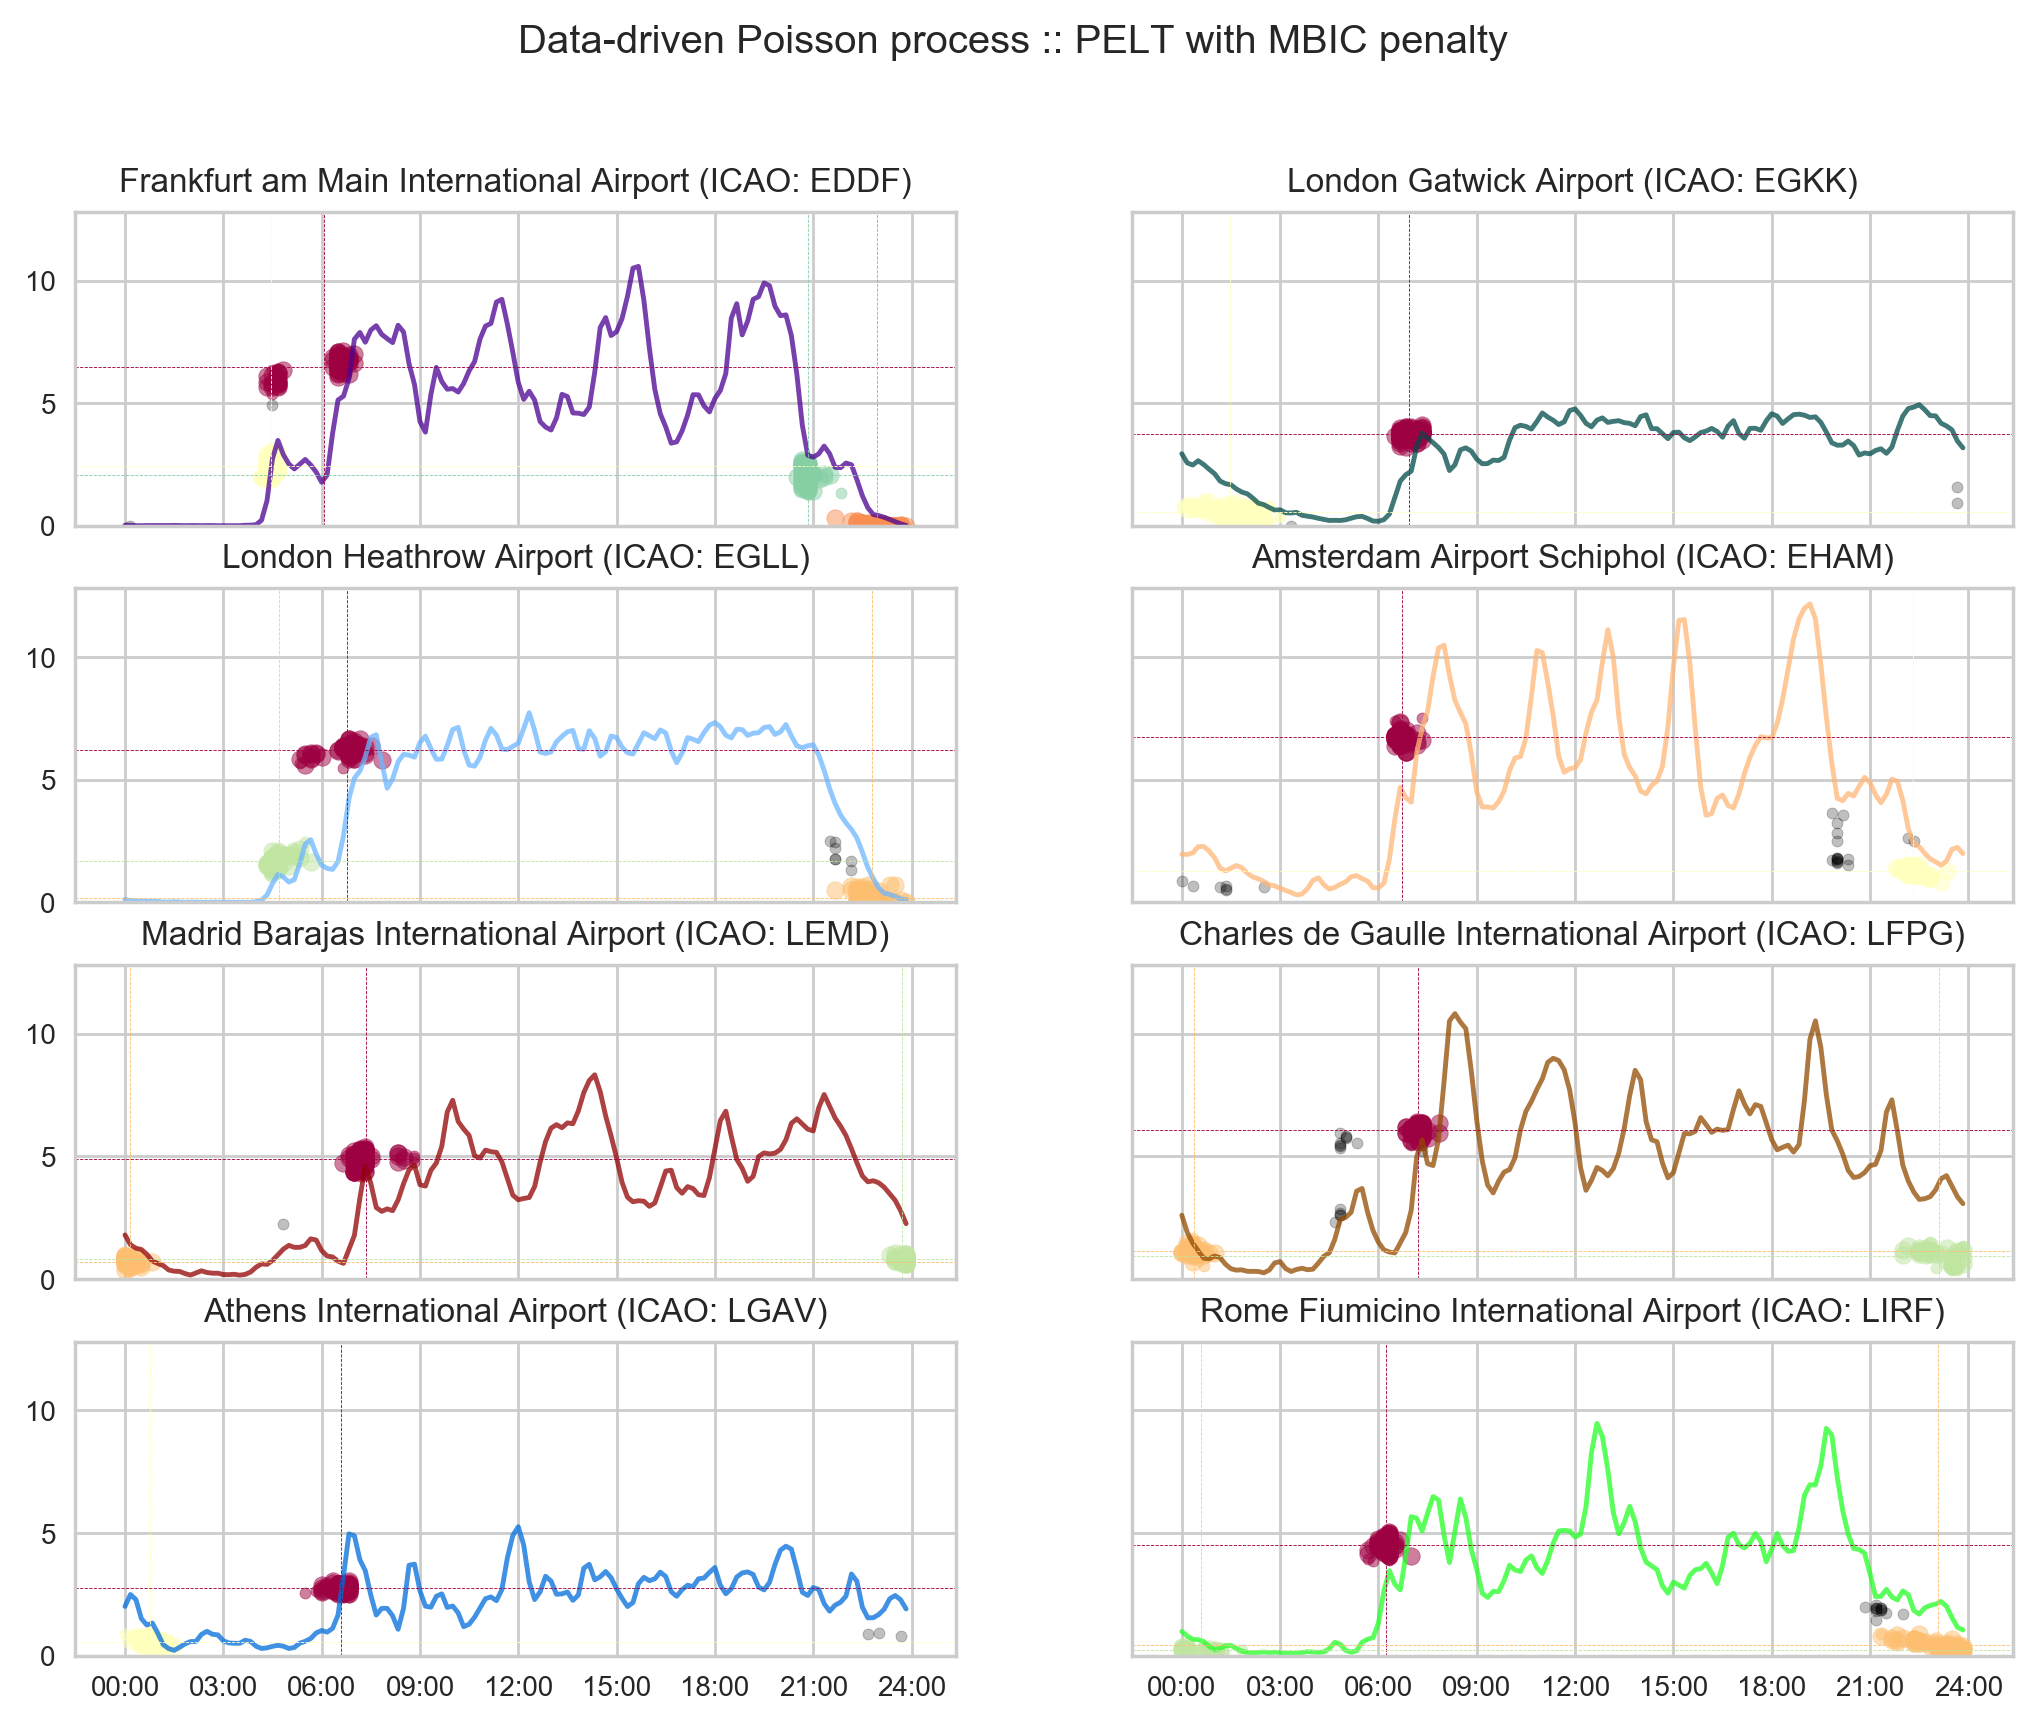
\includegraphics[width=\textwidth]{DDPoisson_MBIC}
      \caption{Data-driven modeling of non-homogeneous Poisson process; \ac{MBIC} penalty. \DBSCAN{} outliers are drawn in black.}\label{fig:DD_MBIC}
  \end{figure}

  Figure~\ref{fig:DD_AIC} shows the change-points identified by \PELT{} and the resulting clustering via \DBSCAN{} when \PELT{} uses the \ac{AIC} penalty.
  In this setting, \PELT{} is much more sensible and detects regime changes in correspondence of maxima and minima of the average demand.
  The resulting description of the arrival stream in terms of a Poisson process is hence richer and follows more closely the average demand.
  However, the increased sensibility in the change point detection comes at the price of a \emph{noisy} distribution of change-points in the \((t,\lambda)\) plane, which might be difficult to reconstruct via \DBSCAN{} (see \airp{lgw}).

  \begin{figure}
      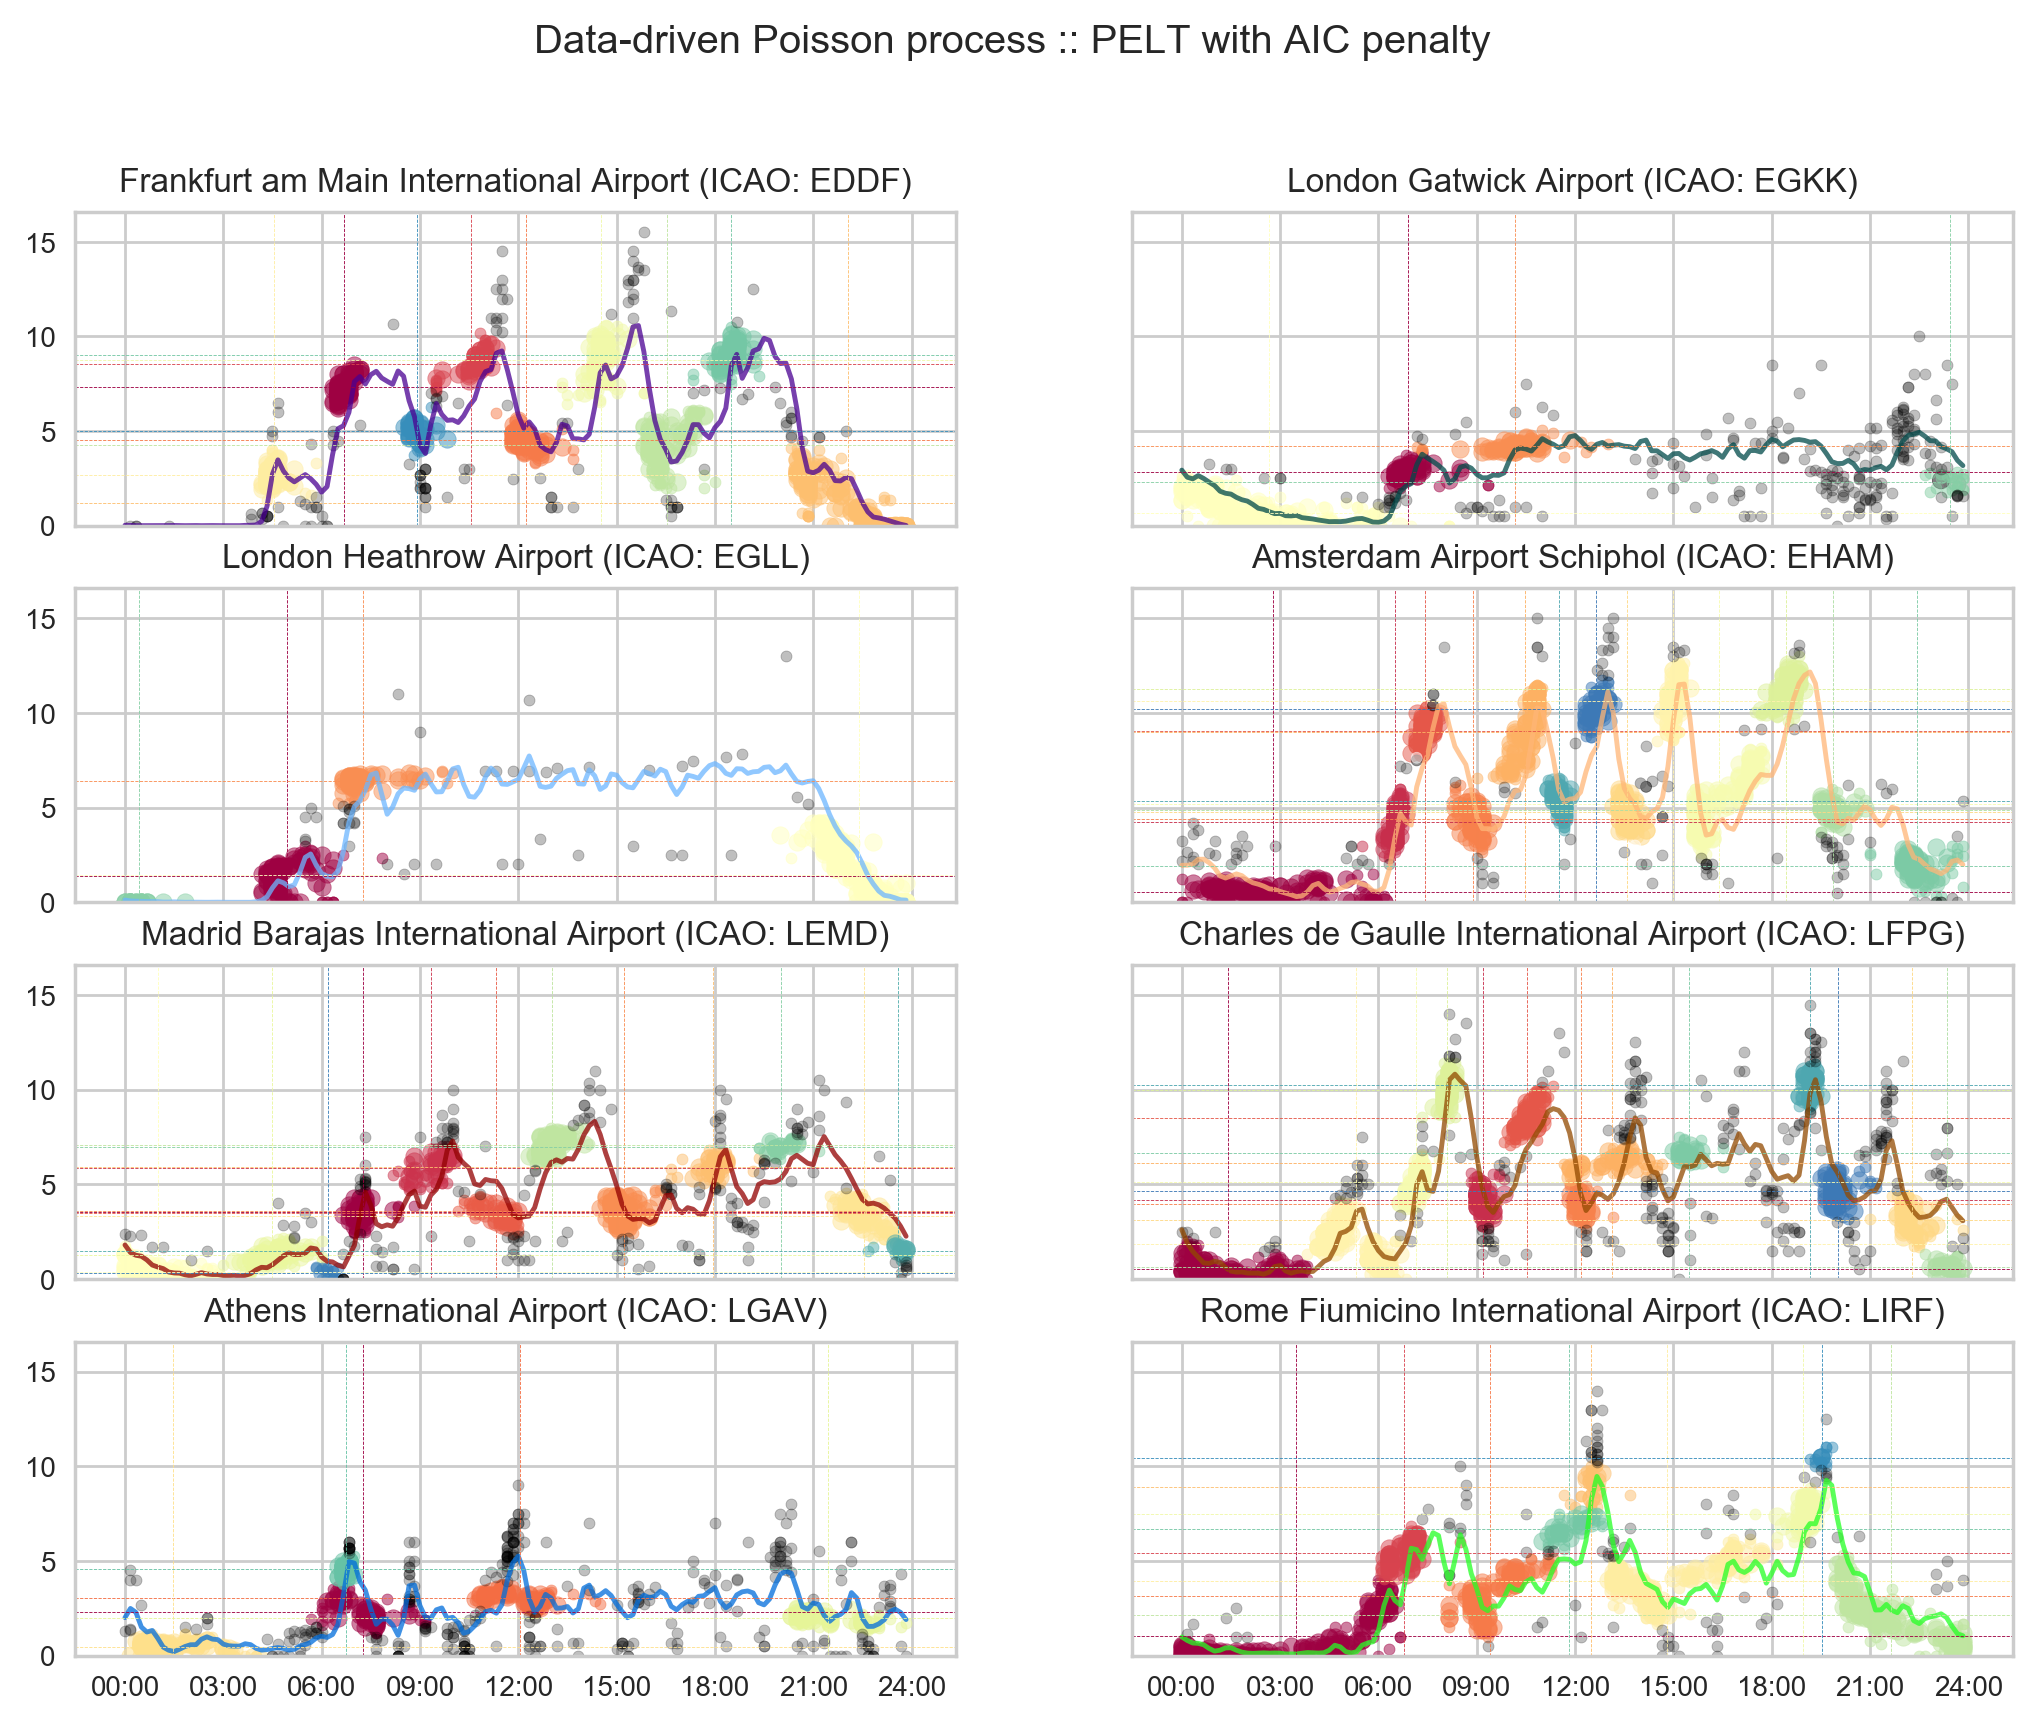
\includegraphics[width=\textwidth]{DDPoisson_AIC}
      \caption{Data-driven modeling of non-homogeneous Poisson process; \ac{AIC} penalty. \DBSCAN{} outliers are drawn in black.}\label{fig:DD_AIC}
  \end{figure}

\section{Continuous wavelet transform of demand time series}\label{sec:appc}

Figure~\ref{fig:cwt} shows a continuous wavelet transform of the demand from the week August 01--07, 2016.
The \(x\)-axis shows the time and the \(y\)-axis shows the scale parameter of the Ricker wavelet. The color bar shows the value of the coefficients of the transform. The plot highlights the presence of a low-frequency component with daily periodicity and high-frequency demand peaks with sufficient regularity, the strength and frequency of which vary across airports.

% replace this with CWT
\begin{sidewaysfigure}
  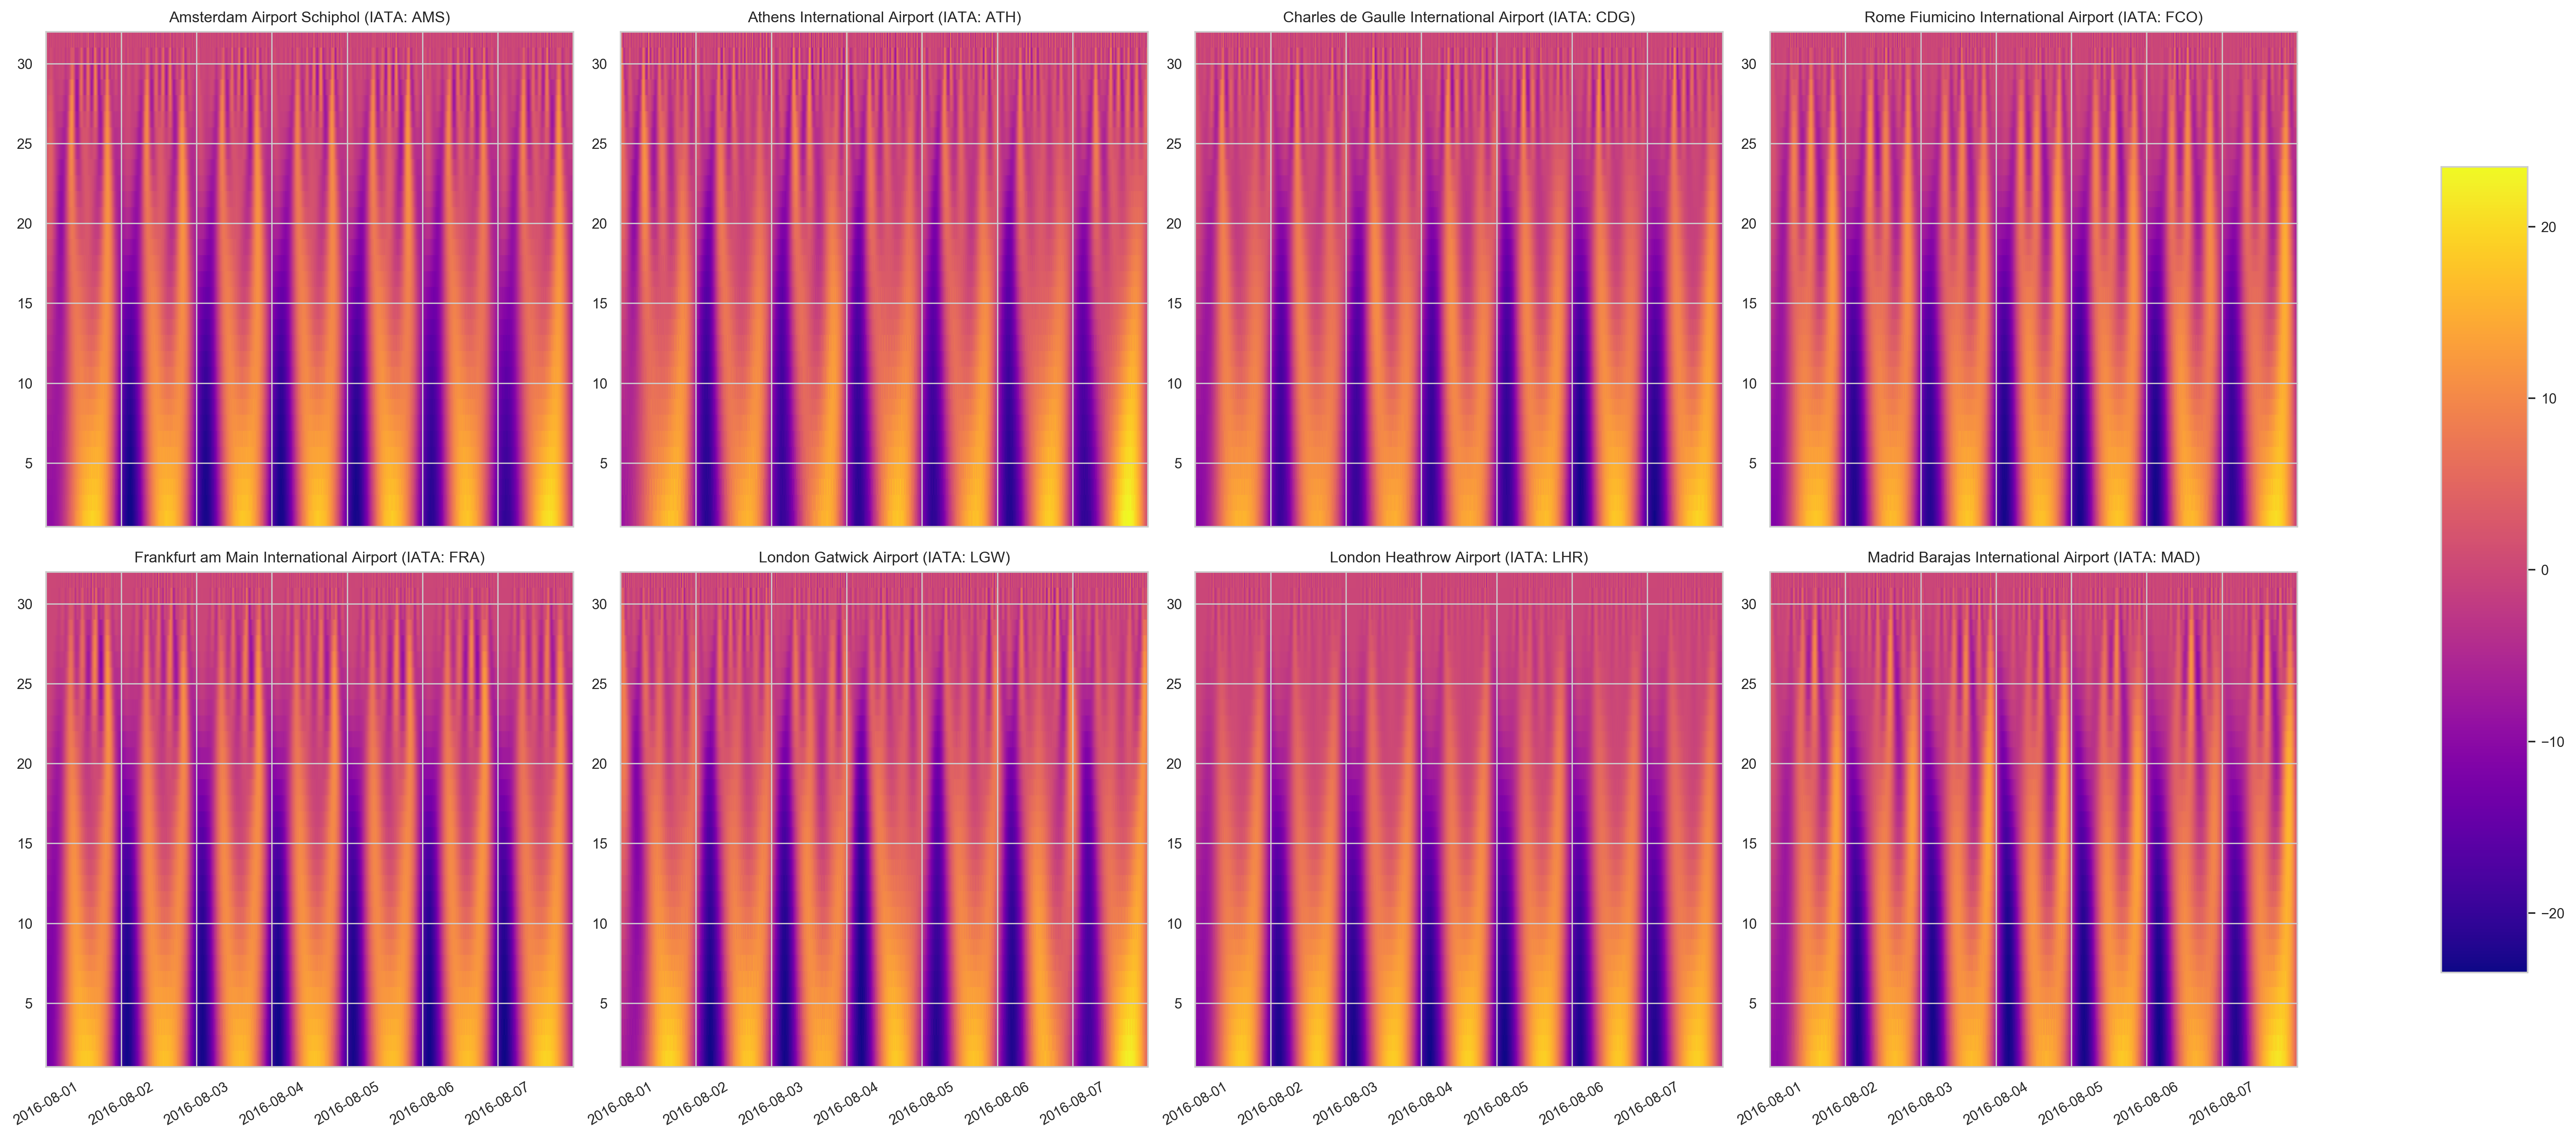
\includegraphics[width=\textwidth]{ContWavltTrasf}
  \caption{Continuous wavelet transform of the demand for the week August 01--07, 2016. The figure clearly shows the presence of a weekly periodic component in the demand at all airports under consideration.}\label{fig:cwt}
\end{sidewaysfigure}

\section{Correlations from regulated flight plan and \acs{PSRA} model}\label{sec:appb}

  Figure~\ref{fig:correlations_psra} shows the Pearson's correlation \(\rho_{t_i, t_{i+1}}\) between the simulated demand variation in the intervals \([t_i, t_{i+1})\) and \([t_{i+1}, t_{i+2})\). The simulated demand variation is obtained by subtracting the demand according to the regulated flight plan \(t^{r}\) from the demand simulated from Model~\eqref{Main-eq:psra-like}.

  Comparing Figures~\ref{Main-fig:correlations_true} and~\ref{fig:correlations_psra}, we observe that the \ac{PSRA} model~\eqref{Main-eq:psra-like} captures this characteristic of the inbound flow very well.

  \begin{sidewaysfigure}
      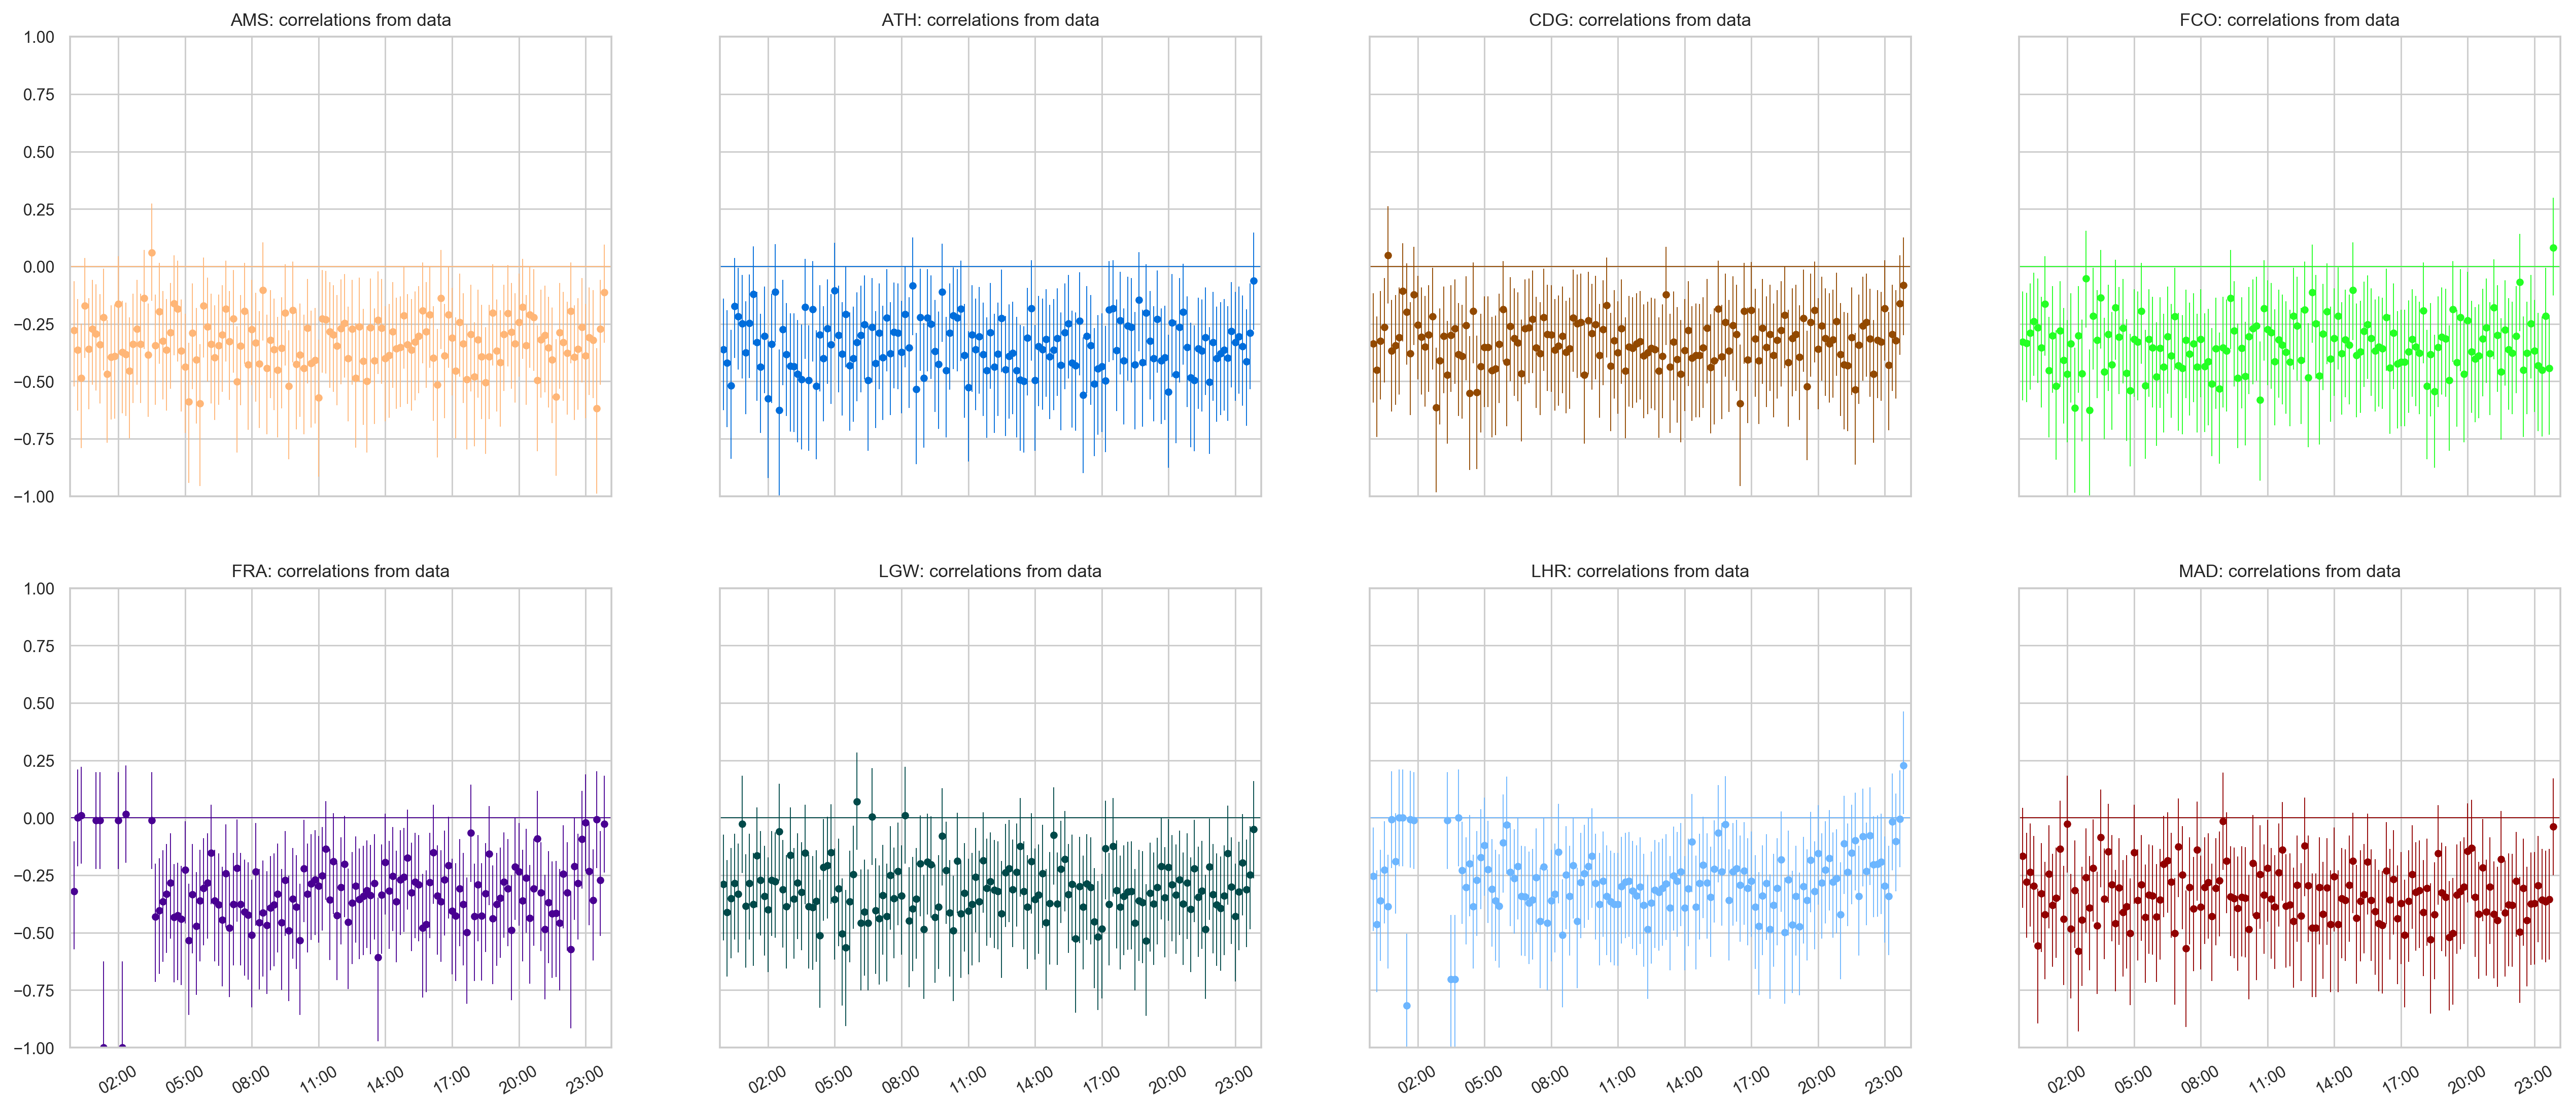
\includegraphics[width=\textwidth]{correlations_psra}
      \caption{Correlations from simulation of Model~\eqref{Main-eq:psra-like}. Error bars show 95\% confidence intervals for Pearson's \(\rho\).}
      \label{fig:correlations_psra}
  \end{sidewaysfigure}

% \clearpage

\section{Intensity function of the data-driven Poisson process}\label{sec:appd}

  This appendix details the intensity function of the Poisson process obtained in Section~\ref{Main-sec:pois}.
  The intensity function is a periodic right-continuous step-function, which takes on value \(\hat{\lambda}\) between two consecutive values of \(\hat{t}\).
  The values of \(\hat{t}\) and \(\hat{\lambda}\) are reported for each airport by Table~\ref{tab:poisson_segmentation} below.
  The table shows how the model correctly captures the typical hourly landing rates in the moments of highest demand, when we expect the airport to operate close to its maximum capacity. For \airp{lhr}, \(\lambda = 0.64\) aircraft/min corresponds to \(38.4\) aircraft/hour, which is close to the maximum declared capacity of 45; for \airp{fra}, \(\lambda = 0.90\) aircraft/min corresponds to \(54\) aircraft/hour, which is close to the maximum declared capacity of 60; finally, for \airp{ams}, \(\lambda = 1.13\) aircraft/min corresponds to \(67.8\) aircraft/hour, which is very close to the the maximum declared capacity of 68 (capacity data from \url{https://ext.eurocontrol.int/airport_corner_public/}).

  \begin{center}
    \begin{longtable}{lll}
      \caption{Non-homogeneous Poisson process derived by \PELT{} and \DBSCAN{} algorithms. The table reports the centroids of the clusters identified by \DBSCAN{} and shown in Figure~\ref{Main-fig:poisson_segmentation}. Times are local.}
      \label{tab:poisson_segmentation}\\

      \toprule
      \multicolumn{1}{c}{airport} & \multicolumn{1}{c}{time} & \multicolumn{1}{c}{\(\lambda\)} \\
      \midrule
      \endfirsthead

      \multicolumn{3}{c}%
      {\tablename\ \thetable{} -- \emph{continued from previous page}} \\
      \toprule
      \multicolumn{1}{c}{airport} & \multicolumn{1}{c}{time} & \multicolumn{1}{c}{\(\lambda\)} \\
      \midrule
      \endhead

      \midrule
      \multicolumn{3}{r}{\emph{Continued on next page}}\\
      \bottomrule
      \endfoot

      \bottomrule
      \endlastfoot

      \airp{fra} & 04:32 UTC+02 &  0.2657 aircraft/min \\
           & 06:41 UTC+02 &  0.7325 aircraft/min \\
           & 08:55 UTC+02 &  0.4991 aircraft/min \\
           & 10:33 UTC+02 &  0.8550 aircraft/min \\
           & 12:14 UTC+02 &  0.4530 aircraft/min \\
           & 14:31 UTC+02 &  0.8757 aircraft/min \\
           & 16:31 UTC+02 &  0.4270 aircraft/min \\
           & 18:29 UTC+02 &  0.9034 aircraft/min \\
           & 22:04 UTC+02 &  0.1182 aircraft/min \\
      \airp{lgw} & 02:40 UTC+01 &  0.0671 aircraft/min \\
           & 06:54 UTC+01 &  0.2858 aircraft/min \\
           & 10:10 UTC+01 &  0.4195 aircraft/min \\
           & 23:26 UTC+01 &  0.2328 aircraft/min \\
      \airp{lhr} & 00:25 UTC+01 &  0.0000 aircraft/min \\
           & 04:56 UTC+01 &  0.1409 aircraft/min \\
           & 07:16 UTC+01 &  0.6410 aircraft/min \\
           & 22:24 UTC+01 &  0.1424 aircraft/min \\
      \airp{ams} & 02:47 UTC+02 &  0.0537 aircraft/min \\
           & 06:30 UTC+02 &  0.4222 aircraft/min \\
           & 07:25 UTC+02 &  0.9062 aircraft/min \\
           & 08:53 UTC+02 &  0.4416 aircraft/min \\
           & 10:28 UTC+02 &  0.9006 aircraft/min \\
           & 11:30 UTC+02 &  0.5334 aircraft/min \\
           & 12:38 UTC+02 &  1.0207 aircraft/min \\
           & 13:35 UTC+02 &  0.4785 aircraft/min \\
           & 15:00 UTC+02 &  1.0653 aircraft/min \\
           & 16:23 UTC+02 &  0.5189 aircraft/min \\
           & 18:26 UTC+02 &  1.1255 aircraft/min \\
           & 19:52 UTC+02 &  0.4881 aircraft/min \\
           & 22:26 UTC+02 &  0.1942 aircraft/min \\
      \airp{mad} & 01:00 UTC+02 &  0.0386 aircraft/min \\
           & 04:30 UTC+02 &  0.1240 aircraft/min \\
           & 06:12 UTC+02 &  0.0293 aircraft/min \\
           & 07:14 UTC+02 &  0.3511 aircraft/min \\
           & 09:19 UTC+02 &  0.5870 aircraft/min \\
           & 11:18 UTC+02 &  0.3470 aircraft/min \\
           & 13:02 UTC+02 &  0.7084 aircraft/min \\
           & 15:14 UTC+02 &  0.3574 aircraft/min \\
           & 17:56 UTC+02 &  0.5905 aircraft/min \\
           & 20:01 UTC+02 &  0.6972 aircraft/min \\
           & 22:33 UTC+02 &  0.3309 aircraft/min \\
           & 23:35 UTC+02 &  0.1493 aircraft/min \\
      \airp{cgd} & 01:24 UTC+02 &  0.0530 aircraft/min \\
           & 05:18 UTC+02 &  0.1852 aircraft/min \\
           & 07:08 UTC+02 &  0.5127 aircraft/min \\
           & 08:06 UTC+02 &  1.0003 aircraft/min \\
           & 09:11 UTC+02 &  0.4170 aircraft/min \\
           & 10:32 UTC+02 &  0.8515 aircraft/min \\
           & 12:11 UTC+02 &  0.3950 aircraft/min \\
           & 13:06 UTC+02 &  0.6116 aircraft/min \\
           & 15:29 UTC+02 &  0.6669 aircraft/min \\
           & 19:09 UTC+02 &  1.0227 aircraft/min \\
           & 20:01 UTC+02 &  0.4632 aircraft/min \\
           & 22:16 UTC+02 &  0.3120 aircraft/min \\
           & 23:21 UTC+02 &  0.0631 aircraft/min \\
      \airp{ath} & 01:27 UTC+03 &  0.0445 aircraft/min \\
           & 06:45 UTC+03 &  0.4592 aircraft/min \\
           & 07:16 UTC+03 &  0.2315 aircraft/min \\
           & 12:03 UTC+03 &  0.3028 aircraft/min \\
           & 21:27 UTC+03 &  0.1993 aircraft/min \\
      \airp{fco} & 03:29 UTC+02 &  0.1019 aircraft/min \\
           & 06:47 UTC+02 &  0.5395 aircraft/min \\
           & 09:24 UTC+02 &  0.3155 aircraft/min \\
           & 11:49 UTC+02 &  0.6698 aircraft/min \\
           & 12:30 UTC+02 &  0.8899 aircraft/min \\
           & 14:48 UTC+02 &  0.3965 aircraft/min \\
           & 18:58 UTC+02 &  0.7465 aircraft/min \\
           & 19:31 UTC+02 &  1.0422 aircraft/min \\
           & 21:37 UTC+02 &  0.2130 aircraft/min \\
    \end{longtable}
  \end{center}

\end{document}
